\chapter{Технологический раздел}

В данном разделе выбраны средства разработки программного обеспечения, показаны детали реализации и способы взаимодействия с программным продуктом.

\section{Средства реализации ПО}
В качестве технологии программирования был выбран объектно-ориен-тированный подход, так как он обеспечивает простую модификацию кода и добавление нового функционала за счёт использования различных паттернов проектирования. 

Для разработки приложения был выбран язык программирования С++. Этот язык подходит для реализации разрабатываемого программного продукта, так как поддерживает парадигму объектно-ориентированного программирования, обеспечивает модульность, раздельную компиляцию, обработку исключений, абстракцию данных, объявление типов (классов) объектов, механизм виртуальности. 

Для связи клиента и сервера по REST-API был использован фреймворк OAT++ \cite{bib:3}, так как он может быть легко встроен в код приложения, кроме того, он предоставляет возможность асинхронной обработки поступающих запросов.

В качестве СУБД была выбрана PostgreSQL \cite{bib:4}, так как она удовлетворяет требованиям, выдвинутым в разделе \ref{subd}. Кроме того, она предоставляет возможность использования индексов. 

В качестве библиотеки доступа к данным была выбрана библиотека SOCI \cite{bib:5}, так как она предоставляет возможность обращения к разным базам данных с минимальным изменением кода (требуется изменить только строку подключения). Кроме того, библиотека предоставляет интерфейс для ORM (Object-Relational-Mapping).

Для реализации графической части приложения был использован фреймворк QT \cite{bib:6}, так как он включает в себя все основные классы, которые могут потребоваться при разработке прикладного программного обеспечения, включая элементы графического интерфейса. 

\section{Архитектура компонентов приложения}
\subsection{Архитектура компонента интерфейса}
Для реализации компонента интерфейса был выбран паттерн MVP, так как он позволяет создать несколько вариантов отображения данных без изменения логики. Так, интерфейс приложения был разработан в 2 вариантах: в графическом и консольном. На рисунке \ref{fig:ui} представлена UML-диаграмма классов компонента интерфейса.

\begin{figure}[H]
	\centering
	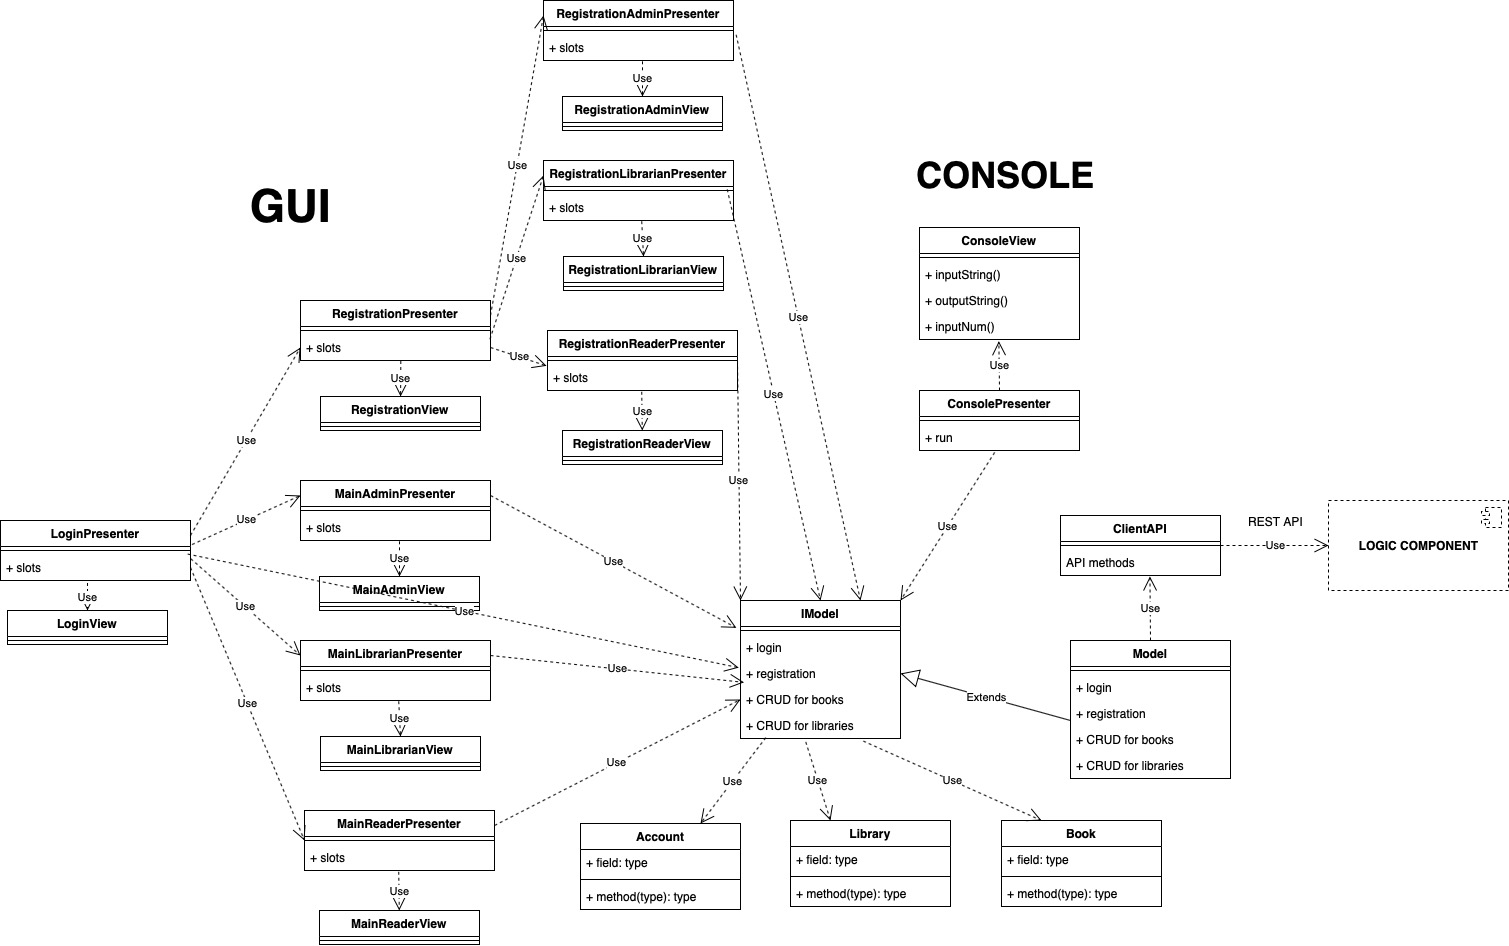
\includegraphics[width = \linewidth]{img/ui.jpg}
	\caption{UML-диаграмма классов компонента интерфейса}
	\label{fig:ui}
\end{figure}

\subsection{Архитектура компонента бизнес-логики}
Компонент бизнес-логики представляет собой REST-API контроллер сервера и класс-менеджер для доступа к данным. На рисунке \ref{fig:bl} представлена UML-диаграмма классов компонента бизнес-логики.

\begin{figure}[H]
	\centering
	\includegraphics[width = \linewidth]{img/Logiс.jpg}
	\caption{UML-диаграмма классов компонента бизнес-логики}
	\label{fig:bl}
\end{figure}

\subsection{Архитектура компонента доступа к данным}
Компонент доступа к данным состоит из следующих наиболее важных классов.
\begin{itemize}
    \item Класс \texttt{Session}, который абстрагирует понятие сессии. Класс является надстройкой над соответсвующим классом библиотеки SOCI.
    \item Класс \texttt{ConnectionPoool}, который представляет собой набор сессий базы данных. Класс является надстройкой над соответсвующим классом библиотеки SOCI.
    \item Классы репозиториев: \texttt{AccountRepository}, \texttt{AdminAccountRepository}, \texttt{LibrarianAccountRepository}, \texttt{ReaderAccountRepository}, \texttt{BookRepo-}\\ \texttt{sitory}, \texttt{LibraryRepository}, которые являются интерфейсом для получения данных о соответствующей сущности из базы. Все репозитории реализуют CRUD-методы (CRUD -- Create \& Remove \& Update \& Delete).
    \item Классы команд (\texttt{AddBookCommand}, \texttt{UpdateLibraryCommand}, и. т. д.).
    
\end{itemize}
На рисунке \ref{fig:db} представлена UML-диаграмма классов компонента доступа к данным.

\begin{figure}[H]
	\centering
	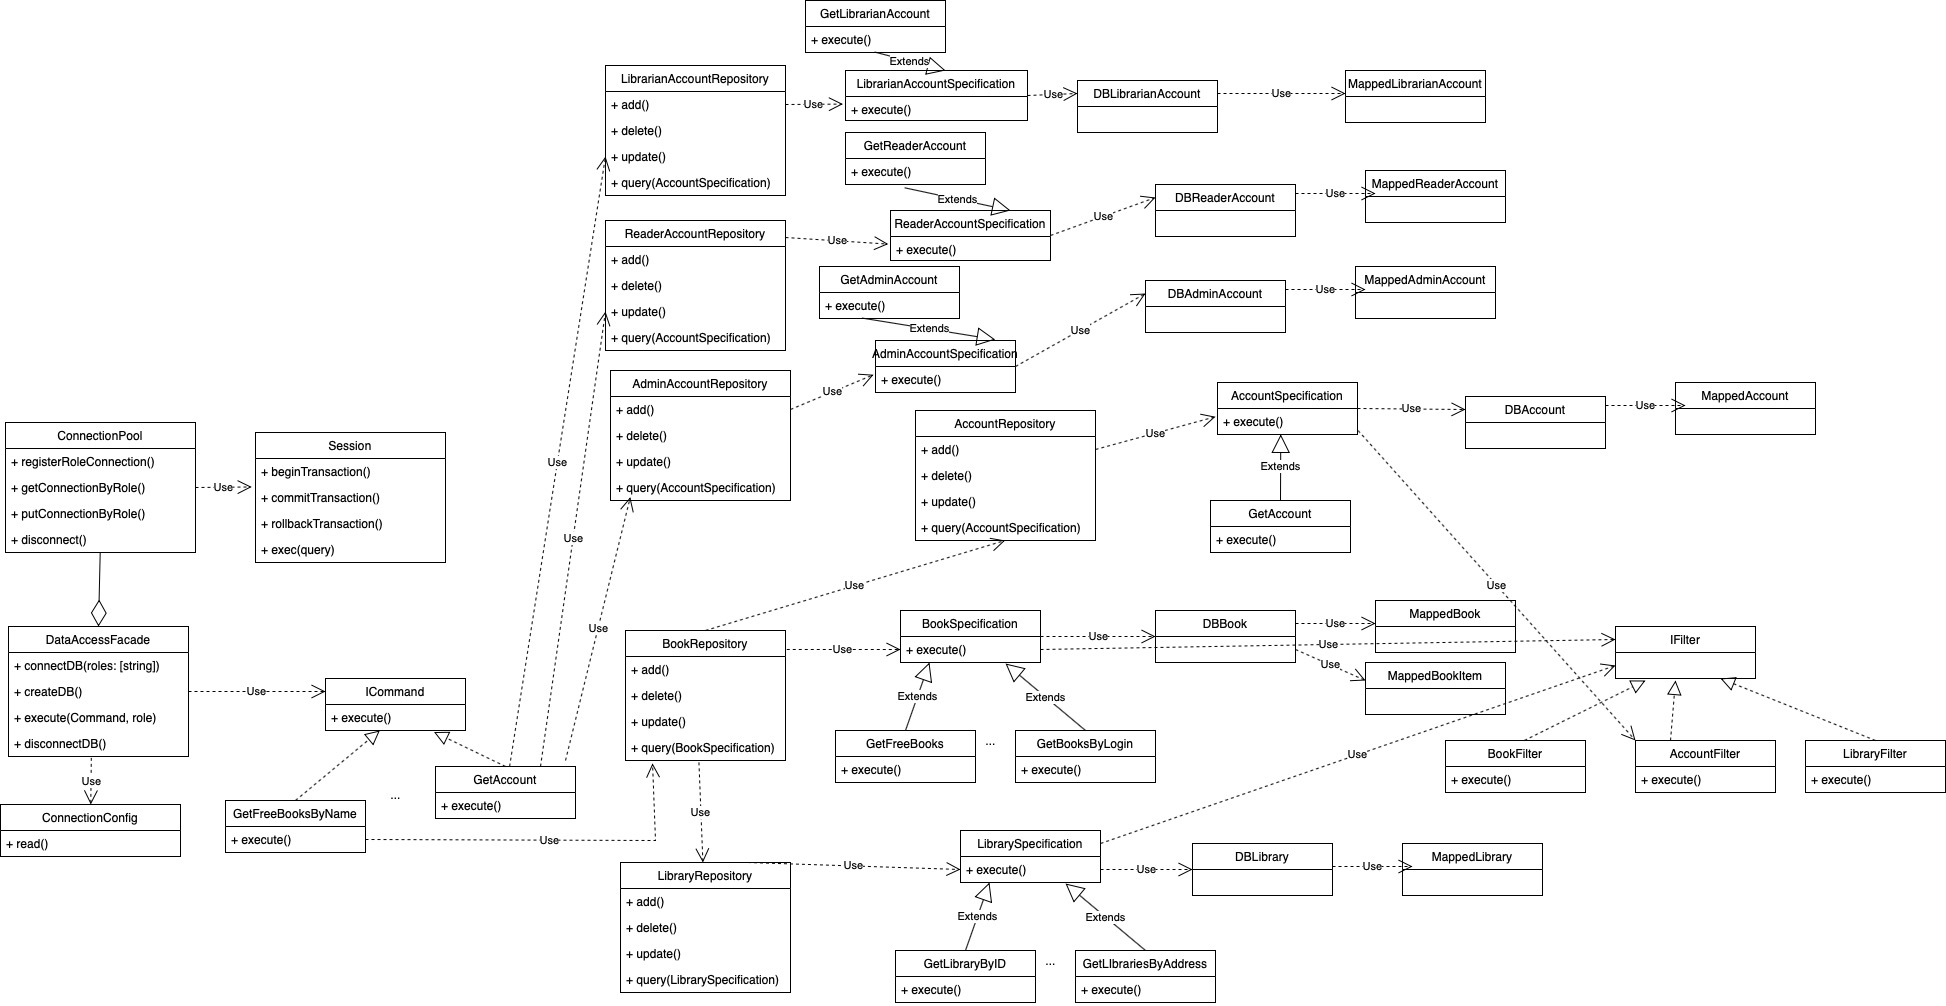
\includegraphics[width = \linewidth]{img/db.jpg}
	\caption{UML-диаграмма классов компонента доступа к данным}
	\label{fig:db}
\end{figure}

\section{Создание объектов БД}
\subsection{Создание таблиц}
В листингах \ref{lst:tableAcc} - \ref{lst:tableBI} приведён код создания таблиц БД. 

Таблица аккаунта каждого пользователя:
\begin{lstlisting}[label=lst:tableAcc, caption=Создание таблицы Account, language=sql]
create table if not exists Account (id serial primary key,
                                    login varchar(30) unique,
                                    password varchar(30),
                                    name varchar(30),
                                    role varchar(30) );
\end{lstlisting}

Таблица, представляющая сущность библиотеки:
\begin{lstlisting}[label=lst:tableLib, caption=Создание таблицы Library, language=sql]
create table if not exists Library (id serial primary key,
                                    name varchar(30),
                                    address varchar(30) );
\end{lstlisting}

Таблица аккаунта библиотекаря:
\begin{lstlisting}[label=lst:tableLAcc, caption=Создание таблицы LibrarianAccount, language=sql]
create table if not exists LibrarianAccount (id serial primary key,
                                             acc_id int references Account(id),
                                             lib_id int references Library(id) );
\end{lstlisting}

Таблица аккаунта администратора:
\begin{lstlisting}[label=lst:tableAAcc, caption=Создание таблицы AdminAccount, language=sql]
create table if not exists AdminAccount (id serial primary key,
                                         acc_id int references Account(id) );
\end{lstlisting}

Таблица аккаунта читателя:
\begin{lstlisting}[label=lst:tableRAcc, caption=Создание таблицы ReaderAccount, language=sql]
create table if not exists ReaderAccount (id serial primary key,
                                          acc_id int references Account(id),
                                          phone varchar(40) );
\end{lstlisting}

Таблица, представляющая дескриптор книги:
\begin{lstlisting}[label=lst:tableBook, caption=Создание таблицы Book, language=sql]
create table if not exists Book (id serial primary key,
                                 name varchar(40),
                                 author varchar(40) );
\end{lstlisting}

Таблица, представляющая экземпляр книги:
\begin{lstlisting}[label=lst:tableBI, caption=Создание таблицы BookItem, language=sql]
create table if not exists BookItem (id serial primary key,
                                     book_id int references Book(id),
                                     lib_id int references Library(id),
                                     acc_id int references Account(id) );
\end{lstlisting}

\newpage
\subsection{Создание триггеров}
В листингах \ref{lst:triggerAcc} - \ref{lst:triggerLib} приведён код создания триггеров БД. 

\noindent DML-триггер, который срабатывает до удаления записи из таблицы Account:
\begin{lstlisting}[label=lst:triggerAcc, caption=Создание триггера (до удаления аккаунта), language=sql]
create or replace function f_delete_acc_trigger()
    returns trigger
as
$$
begin
    update BookItem
    set acc_id = null
    where acc_id = old.id;
    
    return old;
end
$$  language plpgsql;

create or replace trigger bef before delete on Account
    for each row
    execute procedure f_delete_acc_trigger();
\end{lstlisting}

\noindent DML-триггер, который срабатывает до удаления записи из таблицы Library:
\begin{lstlisting}[label=lst:triggerLib, caption=Создание триггера (до удаления библиотеки), language=sql]
create or replace function f_delete_lib_trigger()
returns trigger
as
$$
declare
    ids integer[];
begin
    delete from BookItem
    where lib_id = old.id;

    select into ids array_agg(LibrarianAccount.acc_id)
    from LibrarianAccount join Library on Library.id = lib_id
    where lib_id = old.id;

    delete from LibrarianAccount
    where lib_id = old.id;

    delete from Account
    where id = any(ids);

    return old;
end
$$  language plpgsql;

create or replace trigger bef_lib before delete on Library
    for each row
    execute procedure f_delete_lib_trigger();
\end{lstlisting}

\subsection{Создание функций}
В листингах \ref{lst:funcTake} - \ref{lst:funcReturn} приведён код создания функций БД. 

\noindent Функция взятия книги из библиотеки:
\begin{lstlisting}[label=lst:funcTake, caption=Создание функции взятия книги, language=sql]
create or replace function take_book(login_user varchar, login_lib varchar, bid_p int)
    returns int
as $$
declare
    lid int;
	aid int;
	biid int;
begin
    select into lid max(lib_id)
    from LibrarianAccount join Library on Library.id = lib_id join Account on acc_id = Account.id
    where login_lib = login;

    select into aid max(id)
    from Account
    where login = login_user;

    select into biid min(bookitem.id)
    from bookitem join book on book_id = Book.id
    where bookitem.id = bid_p and lib_id = lid and acc_id is null;

    update bookitem
    set acc_id = aid
    where id = biid;
    return biid;
end;
$$
LANGUAGE PLPGSQL;
\end{lstlisting}
\newpage
\noindent Функция возвращения книги в библиотеку:
\begin{lstlisting}[label=lst:funcReturn, caption=Создание функции возвращения книги, language=sql]
create or replace function return_book(login_user varchar, login_lib varchar, bid_p int)
returns int
as $$
declare
lid int;
	aid int;
	biid int;
begin
    select into lid max(lib_id)
    from LibrarianAccount join Library on Library.id = lib_id join Account on acc_id = Account.id
    where login_lib = login;

    select into aid max(id)
    from Account
    where login = login_user;

    select into biid min(bookitem.id)
    from bookitem join book on book_id = Book.id
    where bookitem.id = bid_p and lib_id = lid and acc_id = aid;

    update bookitem
    set acc_id = null
    where id = biid;
    return biid;
end;
$$
LANGUAGE PLPGSQL;
\end{lstlisting}

\subsection{Создание ролей}

В листингах \ref{lst:roleLib} - \ref{lst:roleReader} приведён код создания ролей БД. 

\noindent Роль библиотекаря с правами на изменение таблицы экземпляров книг и на чтение всех остальных:
\begin{lstlisting}[label=lst:roleLib, caption=Создание ролей, language=sql]
create user librarian WITH PASSWORD 'librarian';
grant select on book, bookitem, account, librarianaccount, library to librarian;
grant update on bookitem to librarian;
\end{lstlisting}

\noindent Роль читателя с правами только на чтение всех таблиц:
\begin{lstlisting}[label=lst:roleReader, caption=Создание ролей, language=sql]
create user reader WITH PASSWORD 'reader';
grant select on book, bookitem, account, readeraccount, library to reader;
\end{lstlisting}


\section{Интерфейс программы}

На рисунках \ref{img:mainadmin} -- \ref{img:mainreader} представлены примеры работы программы.

\begin{figure}[h!]
	\begin{center}
		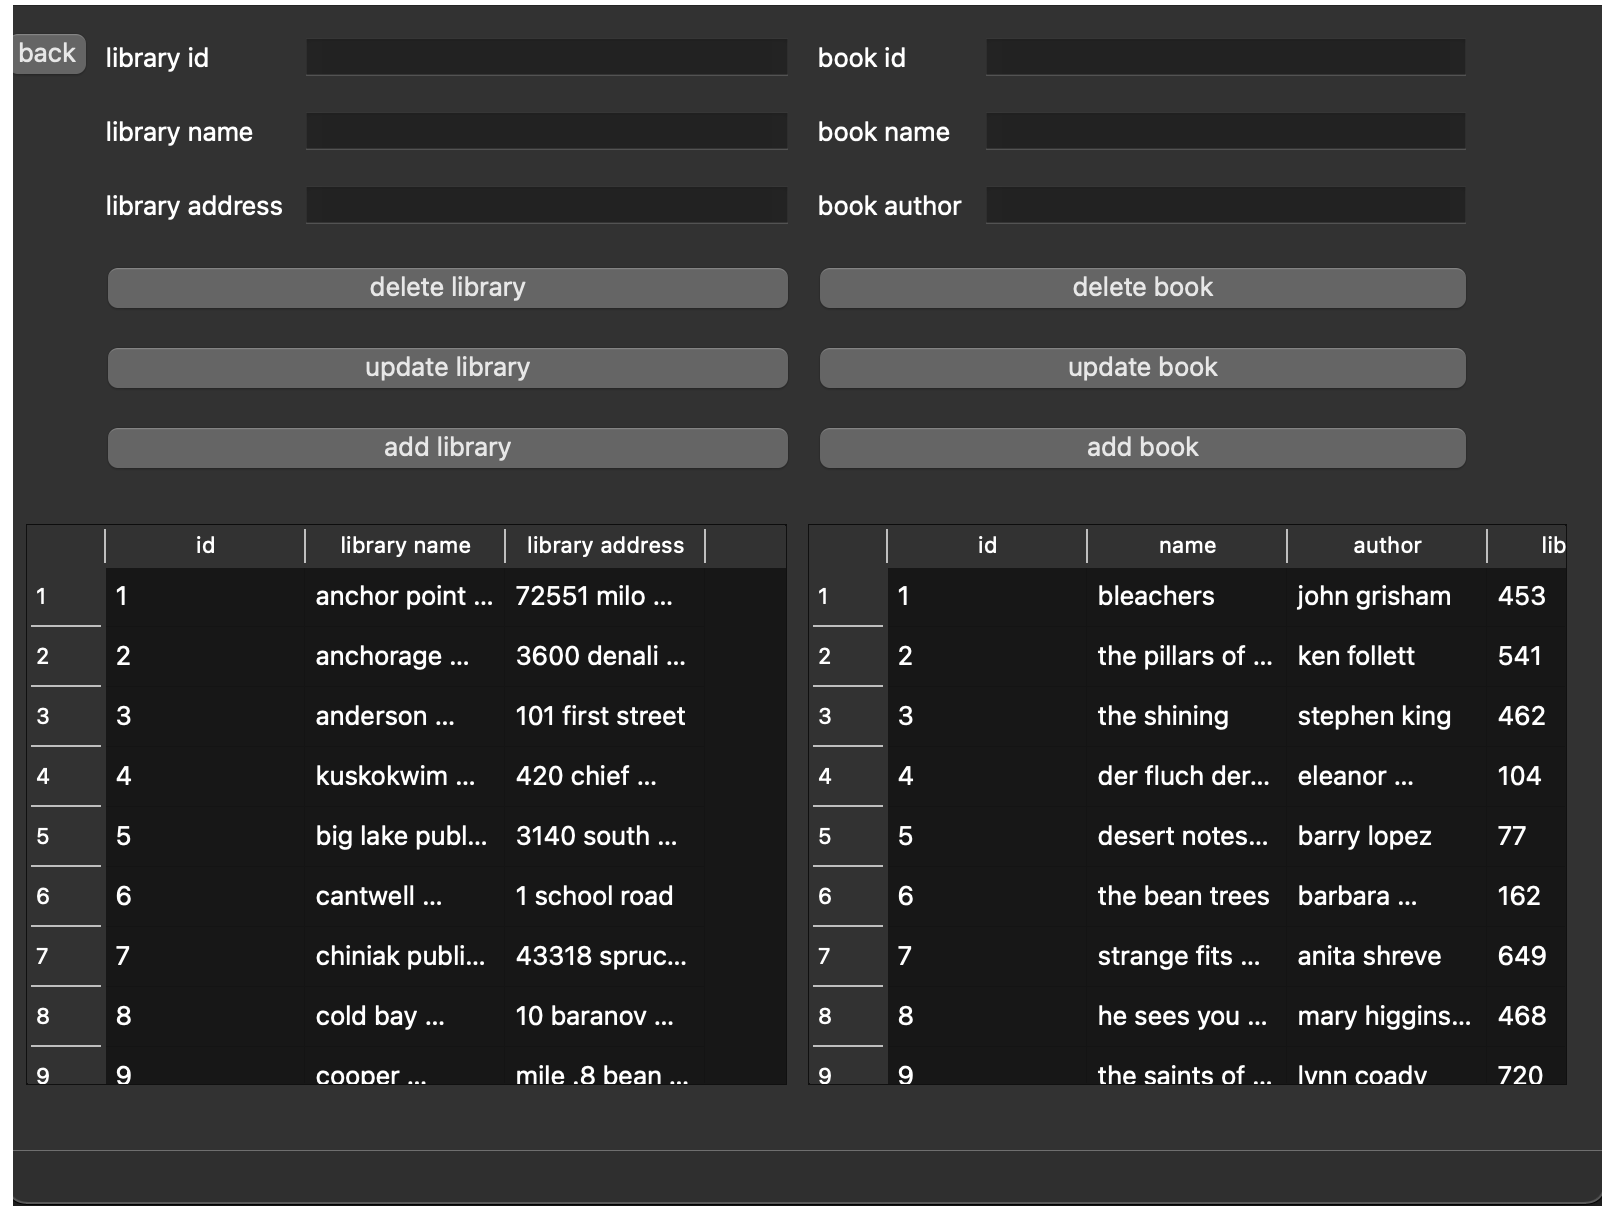
\includegraphics[width = \linewidth]{img/main_admin.png}
	\end{center}
	\captionsetup{justification=centering}
	\caption{Главная страница администратора}
	\label{img:mainadmin}
\end{figure}

\newpage
\begin{figure}[h!]
	\begin{center}
		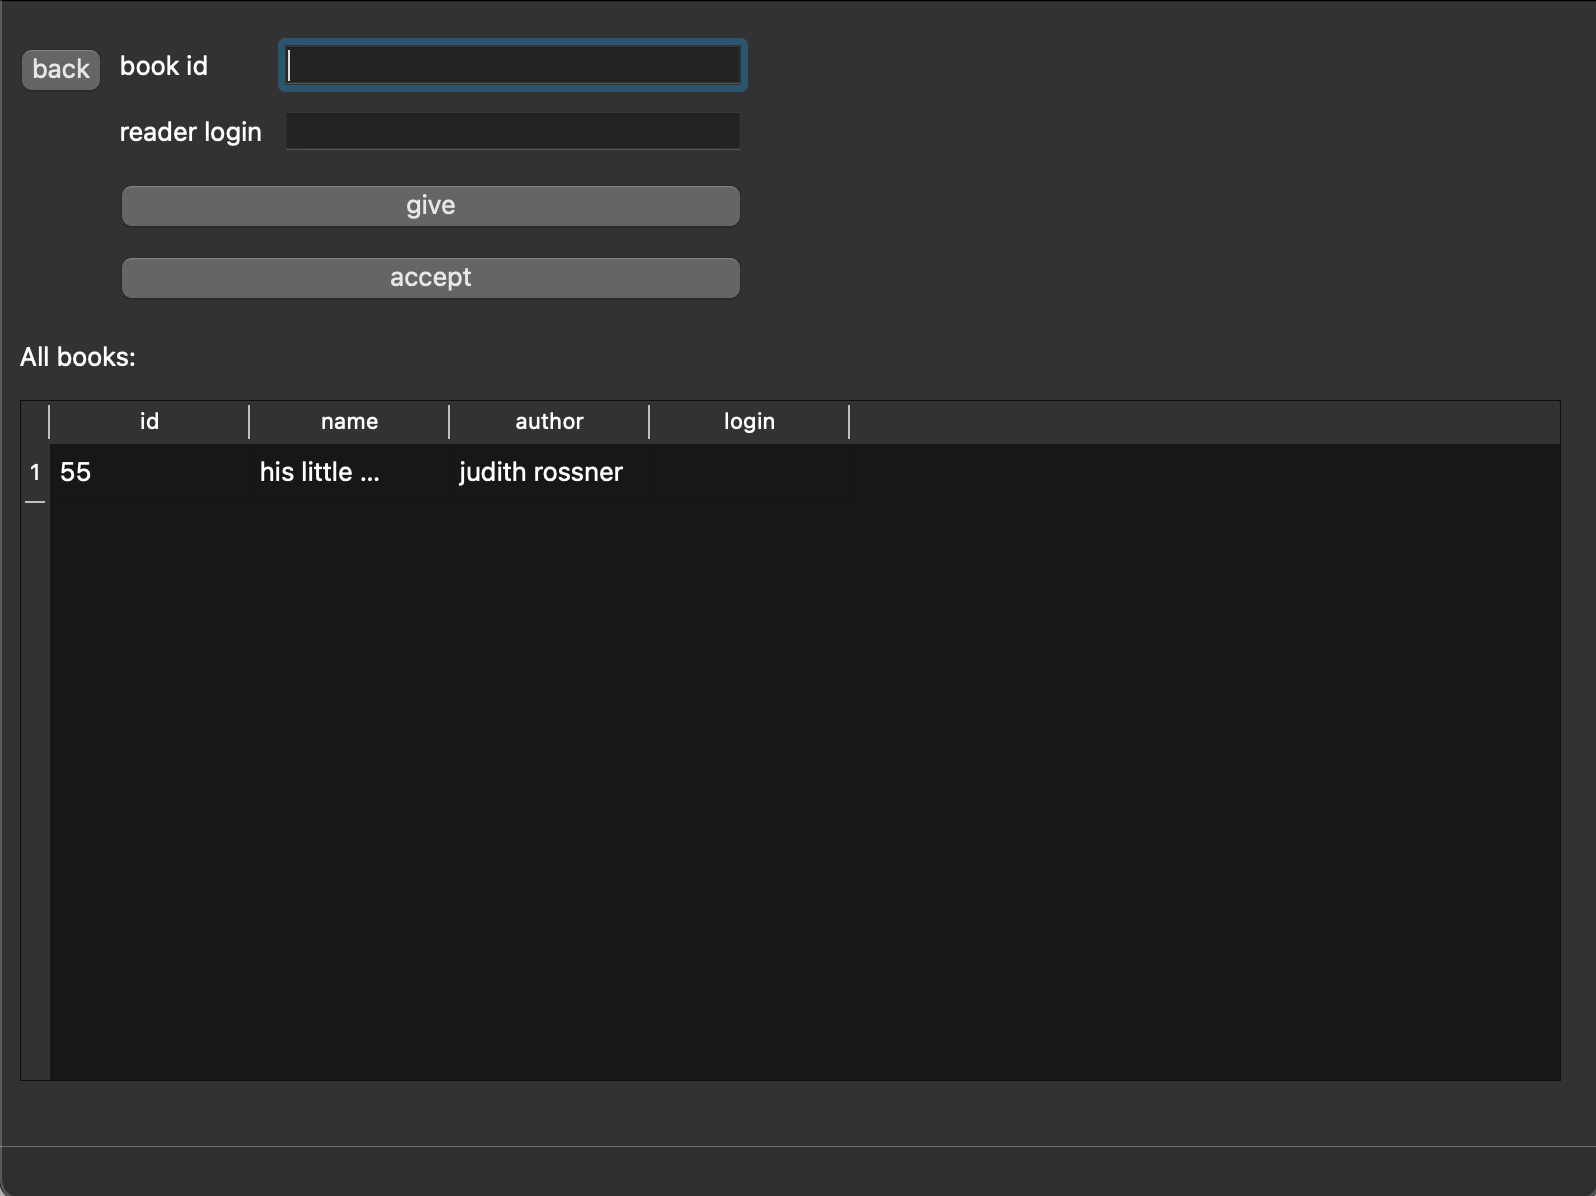
\includegraphics[width = \linewidth]{img/main_librarian.png}
	\end{center}
	\captionsetup{justification=centering}
	\caption{Главная страница библиотекаря}
	\label{img:mainlibrarian}
\end{figure}
\newpage
\begin{figure}[h!]
	\begin{center}
		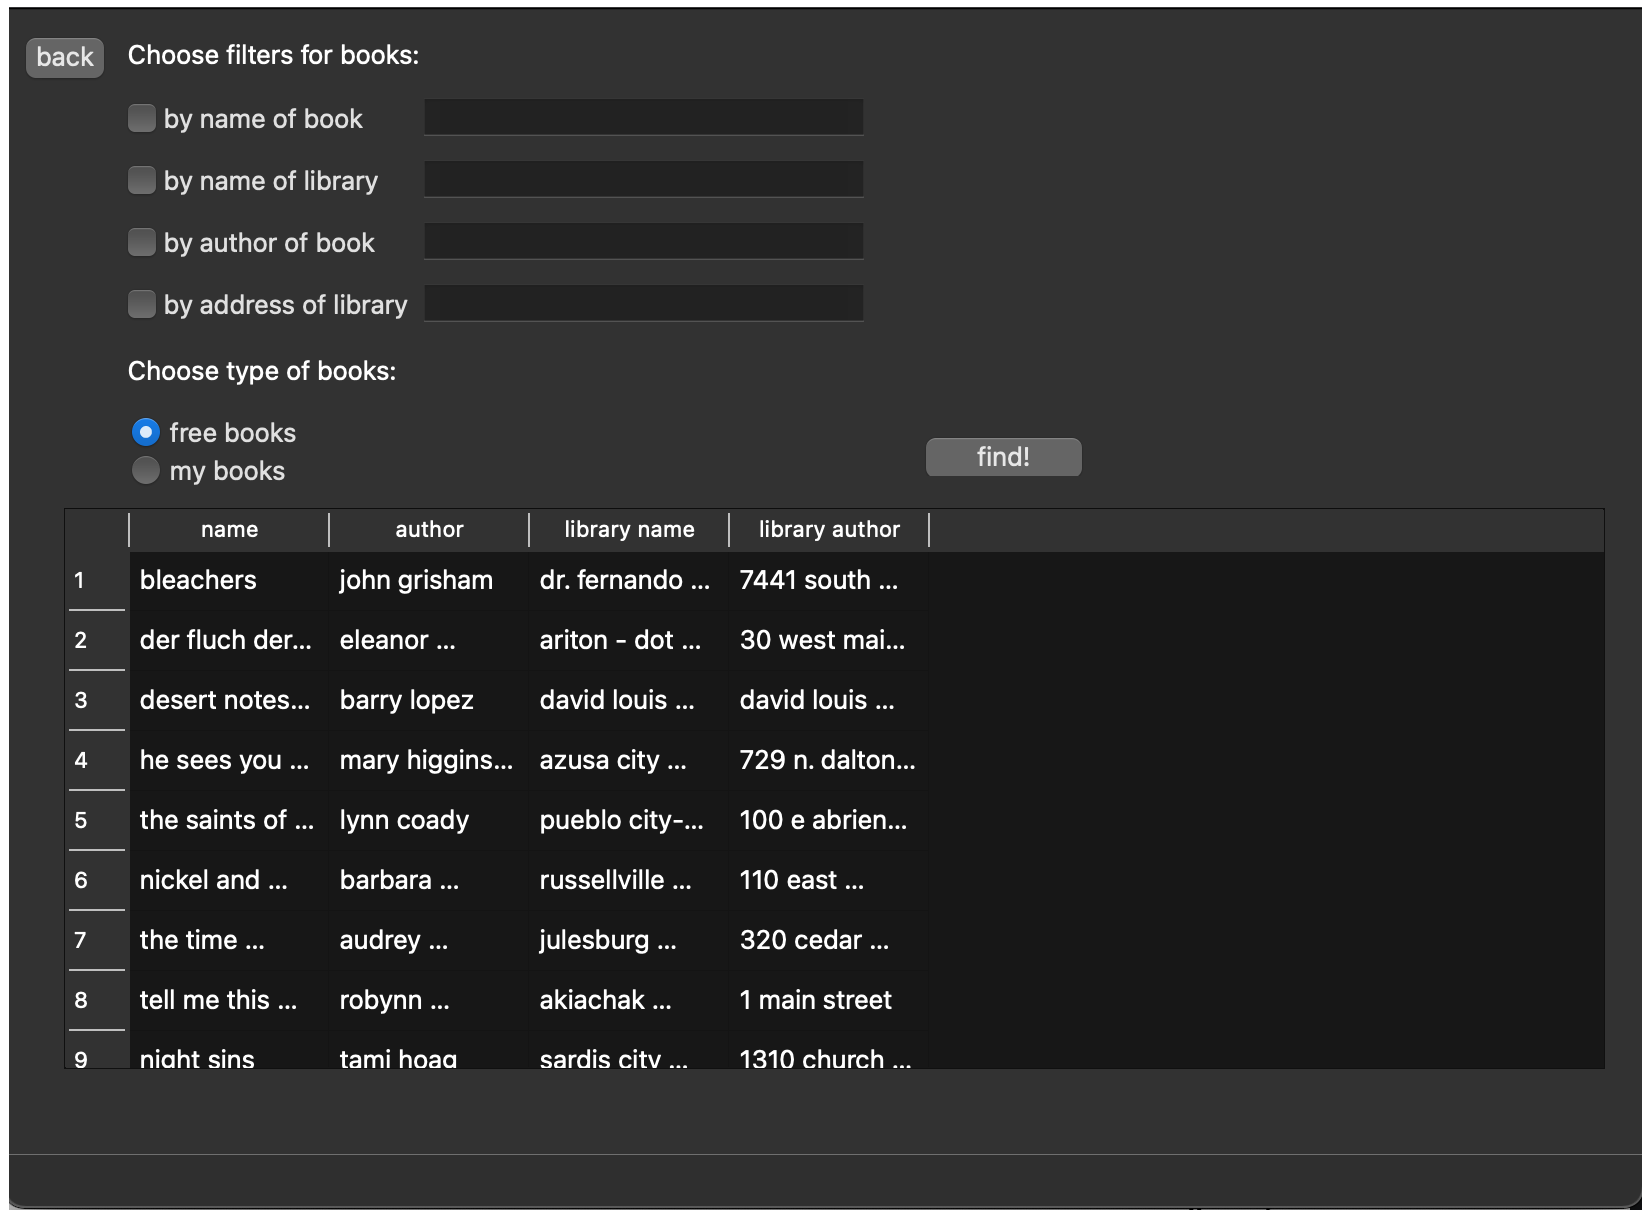
\includegraphics[width = \linewidth]{img/main_reader.png}
	\end{center}
	\captionsetup{justification=centering}
	\caption{Главная страница читателя}
	\label{img:mainreader}
\end{figure}


\section*{Вывод}
\addcontentsline{toc}{section}{Вывод}
В данном разделе были выбраны средства разработки программного обеспечения, показаны детали реализации и способы взаимодействия с программным продуктом.